\documentclass[11pt,aspectratio=169]{beamer}

% Assets
\usepackage[czech]{babel}				% Jazyk
\usepackage[a-2u]{pdfx}					% Kopírování z pdfka
\usepackage{tikz}						% Schémata automatů
\usepackage{csquotes}					% české uvozovky
\usepackage{enumerate}					% enumerate environment
\usepackage{indentfirst}
\usepackage{mathtools}
\usepackage{pifont}
\usepackage{xcolor}
\usepackage{enumitem,xcolor}
\usepackage{amsmath}
\usepackage[utf8]{inputenc}

\usepackage{listings}                   % Úryvky z kódu (C#)
\lstset{language=[Sharp]C, frame=lr}
% Enumerate
%\setlist[enumerate]{topsep=0pt,itemsep=-1ex,partopsep=1ex,parsep=1ex,label=(\arabic*)}

\MakeOuterQuote{"}

% Colors
\definecolor{lightblue}{HTML}{009AD4}
\definecolor{darkgreen}{HTML}{0D7103}
\definecolor{lightgreen}{HTML}{68FF00}
\definecolor{darkred}{HTML}{AF0B0B}
\definecolor{lightred}{HTML}{FF5100}
\definecolor{orange}{HTML}{FFE000}
\definecolor{codeblue}{HTML}{FF0055}
\definecolor{codegreen}{rgb}{0,0.6,0}
\definecolor{codegray}{rgb}{0.5,0.5,0.5}
\definecolor{codebeige}{HTML}{D4A000}
\definecolor{backcolour}{rgb}{0.95,0.95,0.92}

\newcommand{\markred}[1]{\textcolor{lightred}{#1}}
\newcommand{\markgreen}[1]{\textcolor{lightgreen}{#1}}
\newcommand{\markorange}[1]{\textcolor{orange}{#1}}
\newcommand{\markblue}[1]{\textcolor{lightblue}{#1}}

% Inline images
\newcommand{\inlineimgscale}{1.1}

% X and check mark
\newcommand{\cmark}{\markgreen{\ding{51}}}
\newcommand{\xmark}{\markred{\ding{55}}}

% Redefinions
\renewcommand{\implies}{\Rightarrow}
\renewcommand{\impliedby}{\Leftarrow}

% Math
\newcommand{\R}{\mathbb{R}}
\newcommand{\C}{\mathbb{C}}
\newcommand{\N}{\mathbb{N}}
\newcommand{\Z}{\mathbb{Z}}
\newcommand{\Q}{\mathbb{Q}}

% Code
\lstdefinestyle{clang}{
    basicstyle=\small\ttfamily\color{white},
    language=C,
    keywordstyle=\color{codeblue},
    commentstyle=\color{codegreen},
    numberstyle=\tiny\color{codegray},
    stringstyle=\color{codebeige},
    breakatwhitespace=false,
    breaklines=true,
    captionpos=b,
    keepspaces=true,
    numbersep=5pt,
    showspaces=false,
    showstringspaces=false,
    showtabs=false,
    morekeywords={void,int,double,float,unsigned,if,else,\#include}
    tabsize=0.5
}
\lstset{escapeinside={(*}{*)},style=clang}

\newcommand{\hlcode}[1]{\colorbox{red}{#1}}
% Beamer theme
\usetheme{Boadilla}
\setbeamertemplate{frame numbering}[fraction]
\usecolortheme[named=black]{structure}
\setbeamertemplate{navigation symbols}{}
\setbeamerfont{title}{series=\bfseries,parent=structure}
\setbeamerfont{frametitle}{series=\bfseries,parent=structure}
\usefonttheme[onlymath]{serif}
\urlstyle{same}

% Dark theme
\setbeamercolor{frametitle}{fg=white}
\setbeamercolor{title}{fg=white}
\setbeamercolor{background canvas}{bg=black}
\setbeamercolor{normal text}{fg=white}

\defbeamertemplate*{title page}{customized}[1][]
{ 
  \usebeamerfont*{title}\inserttitle\par
  \bigskip
  \usebeamerfont*{subtitle}\textit{\insertsubtitle}\par
  \bigskip \bigskip \bigskip \bigskip 
  \usebeamerfont{author}\insertauthor\par
  \usebeamerfont{institute}Kabinet \office\\\url{weber3@spsejecna.cz}\bigskip
}

% Title page
\title{Algoritmizace}
\def\spacing{0.7em}
\def\bigspacing{5em}

\begin{titlepage}
    \begin{center}
        \vspace*{\fill}
        \Huge{\textbf{\maintitle}}\\
        \huge{\subtitle}\\
        \vspace*{\spacing}
        \large{\textbf{\authorname}}\\
        \vspace*{\spacing}
        \large{\textsc{\institution}}\\
        \vspace*{\bigspacing}
        \vspace*{\fill}
        \large{\textit{Poslední aktualizace:} \currentdate}
    \end{center}
    \pagenumbering{arabic}
    \normalsize
\end{titlepage}

\begin{document}

    % Slides
    \begin{frame}
        \titlepage
    \end{frame}

    \section{Tvorba programu}

    \subsection{Algoritmizace}
    \begin{frame}[t]{Algoritmizace}
        \only<2->{Chci něco spočítat, jak na to?}
        \only<3->{
        \begin{itemize}
            \only<3->{\item Rozmyslím si postup výpočtu}
            \only<4->{\item Provedu výpočet podle vymyšleného postupu}
        \end{itemize}
        }
        \only<5->{Potřebuji nutně rozumnět postupu?}
        \only<6->{\begin{center}
            \markred{$\implies$ Nepotřebuji, důležitá je jeho správnost!}
        \end{center}}
    \end{frame}

    \subsection{Algoritmus}
    \begin{frame}{Algoritmus}
        \only<2>{\begin{block}{Co je to algoritmus?}
            Přesný návod či postup, kterým lze vyřešit daný typ úlohy.
        \end{block}}
    \end{frame}
    \begin{frame}[t]{Algoritmus}
        \only<2->{V užším slova smyslu se algoritmem rozumí takové postupy, které mají určité vlastnosti.}
        \only<3->{
            \begin{block}{Vlastnosti algoritmu}
                \begin{itemize}
                    \item \textbf{Elementárnost (diskrétnost).} Algoritmus se skládá z konečného počtu jednoduchých (elementárních) kroků.
                    \only<4->{\item \textbf{Konečnost (finitnost).} Algoritmus musí skončit v konečném počtu kroků.}
                    \only<5->{\item \textbf{Obecnost (hromadnost).} Algoritmus neřeší jeden konkrétní problém, ale obecnou třídu obdobných problémů (např. neřeší jen "kolik je $2\cdot 2$", ale obecně součin libovolné dvojice čísel $a\cdot b$).}
                    \only<6->{\item \textbf{Determinovanost.} Po každém kroku lze jednoznačně určit, který následuje.}
                    \only<7->{\item \textbf{Správnost.} Algoritmus řeší danou úlohu, tj. pro přípustná data vydá správný výsledek a nesprávná vstupní data zamítne.}
                \end{itemize}
            \end{block}
        }
    \end{frame}

    \subsection{Záznam algoritmu}
    \begin{frame}[t]{Záznam algoritmu}
        \only<2->{Každý záznam (popis) algoritmu musí být}
        \only<3->{
            \begin{itemize}
            \only<3->{\item \textbf{Srozumitelný.} Je jasné, co a jak algoritmus řeší.}
            \only<4->{\item \textbf{Přehledný.} Ze záznamu je algoritmus rychle uchopitelný.}
            \only<5->{\item \textbf{Jednoznačný.} Každý krok musí být jednoznačně popsán (vágní popisy jsou nežádoucí).}
            \only<6->{\item \textbf{Stručný.} Neuvádíme zbytečné detaily (matoucí).}
            \end{itemize}
        }
    \end{frame}
    \subsection{Záznam algoritmu}
    \begin{frame}[t,fragile]{Způsoby zadání algoritmu}
        \only<2->{\begin{enumerate}
            \only<2->{\item Slovním vyjádřením $\implies$ např. tzv. \textbf{pseudokódem}.}
            \only<3->{\begin{exampleblock}{Příklad pseudokódu}
                1. Vytvoř proměnnou $x$\\
                2. Pro $i=1,2,\dots,10$ opakuj:\\
                3. \;\;\;Do $x$ ulož hodnotu $x+i$\\
                4. Vypiš hodnotu proměnné $x$
            \end{exampleblock}}
            \only<4->{\markred{$\implies$ Pozor, zde je obvzlášť třeba dbát na jednoznačný zápis!}}
            \only<5->{\item Smluveným grafickým vyjádřením (diagramem)}
            \only<6->{\begin{block}{Druhy diagramů}
                \begin{itemize}
                    \item \textbf{Plošný strukturogram} (tzv. "blokáč")
                    \item \textbf{Vývojový diagram}
                \end{itemize}
            \end{block}}
        \end{enumerate}}
    \end{frame}

    \section{Diagramy}

    \subsection{Prvky algoritmu}
    \begin{frame}[t]{Prvky algoritmu}
        \only<2->{\begin{itemize}
            \setlength\itemsep{1em}
            \only<2->{\item \textbf{Sekvence.} Jednotlivý krok, vykoná se vždy.}
            \only<3->{\item \textbf{Selekce.} Větvení programu, volba pokračování dle stanovené podmínky.}
            \only<4->{\item \textbf{Iterace.} Cyklus, tj. opakované provádění určité posloupnosti příkazů, dokud je splněna stanovaná podmínka.
            \begin{itemize}
                \item Iterace \emph{s testem na začátku}
                \item Iterace \emph{s testem na konci}
            \end{itemize}}
        \end{itemize}}
    \end{frame}

    \subsection{Značky}

    \subsubsection{Sekvence}
    \begin{frame}{Sekvence}
        Činnosti jsou vykonávány v pořadí od shora dolů.
        \begin{columns}
            \begin{column}{.5\textwidth}
                \begin{figure}
                    \centering
                    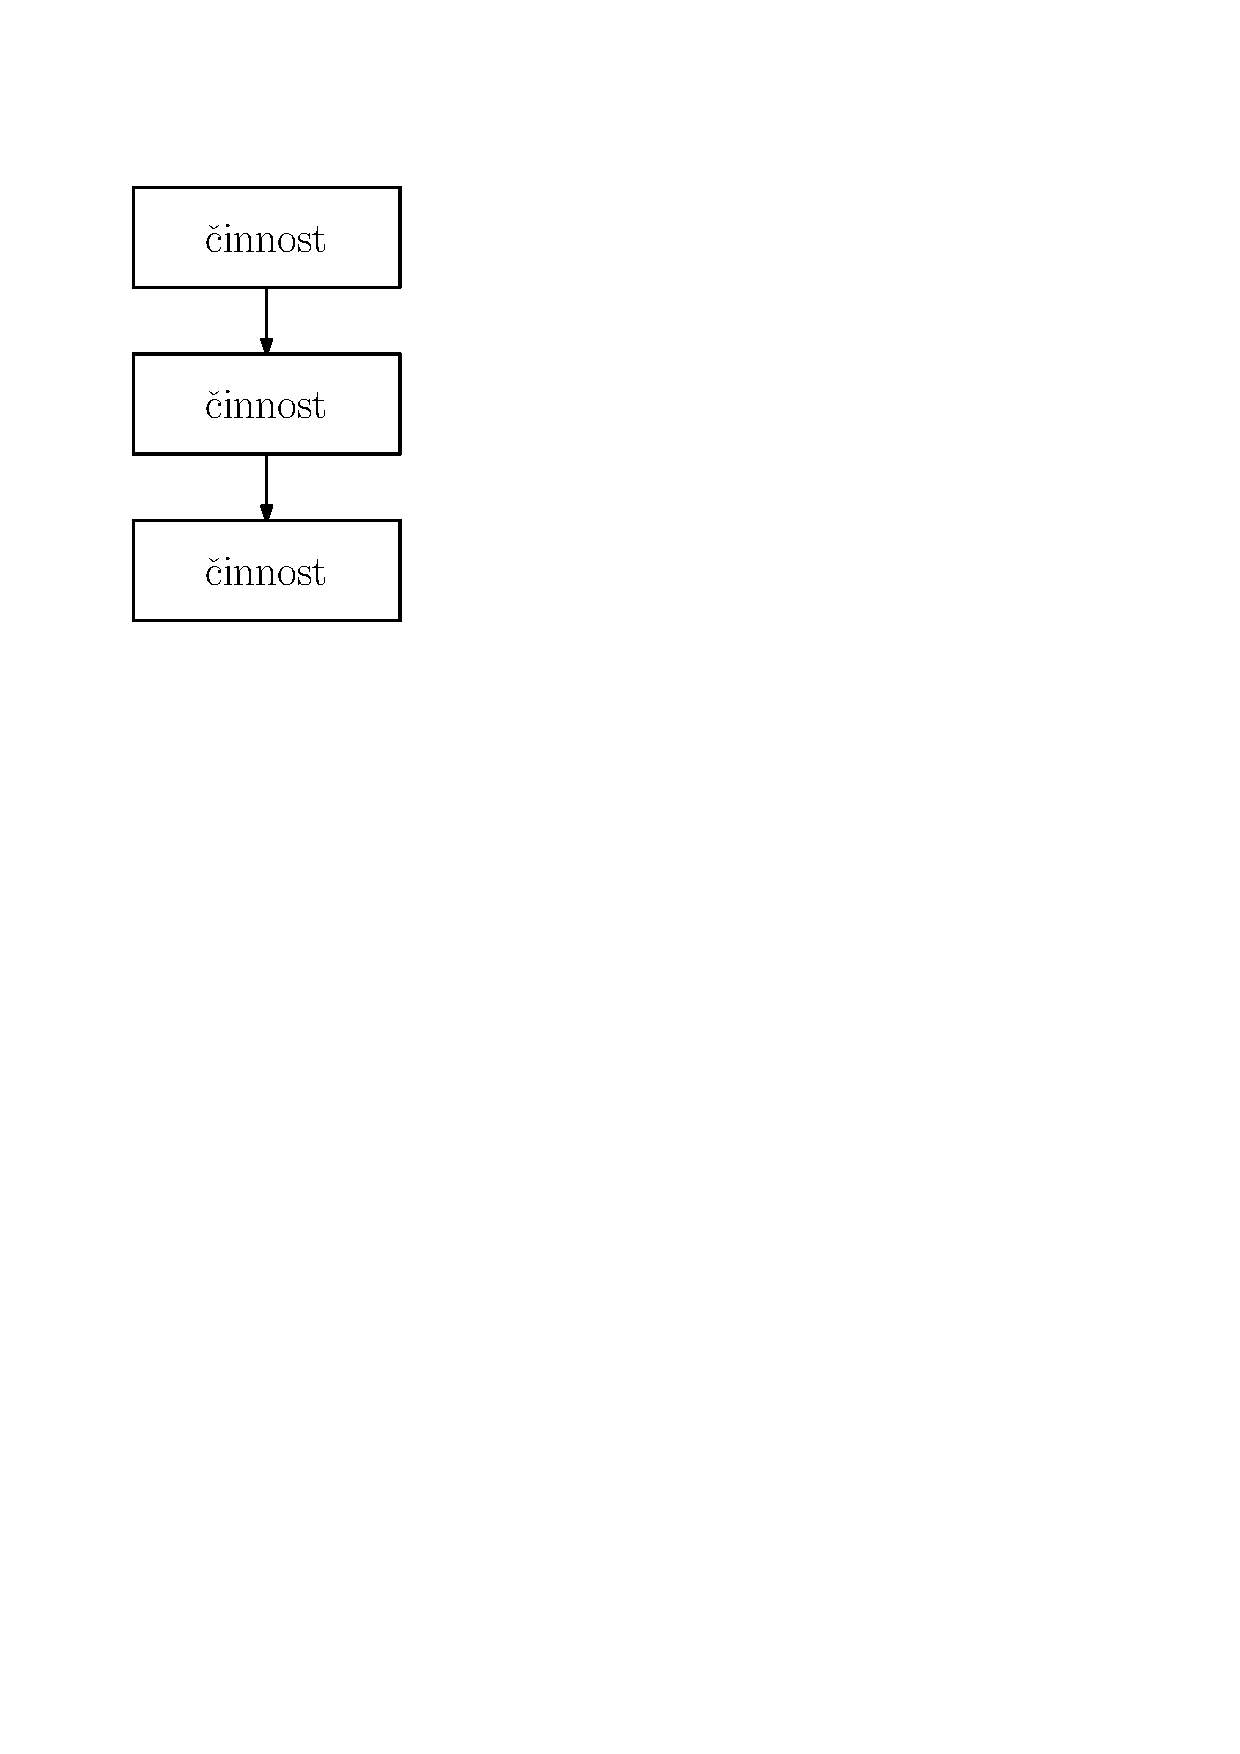
\includegraphics[scale=.6]{../images/00-vyvojak-sekvence.pdf}
                \end{figure}
            \end{column}
            \begin{column}{.5\textwidth}
                \begin{figure}
                    \centering
                    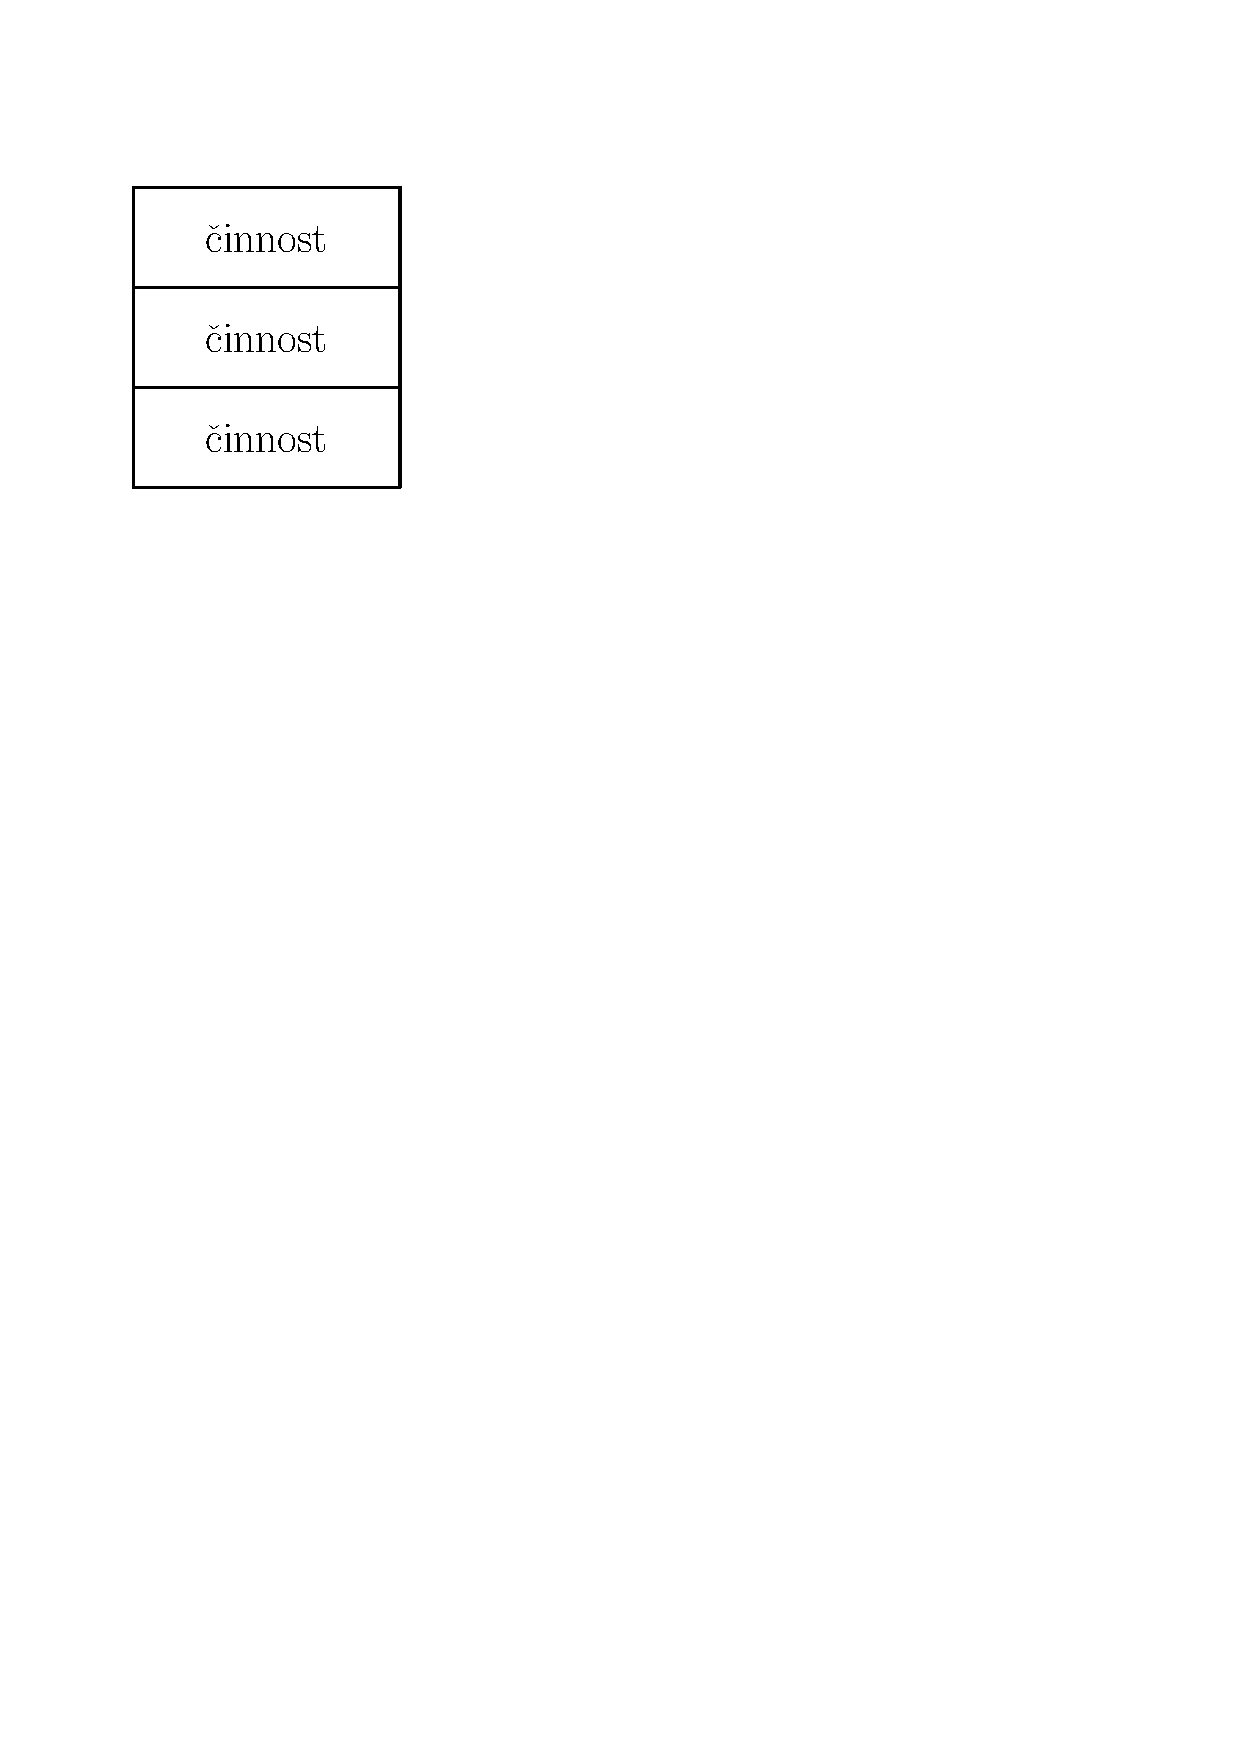
\includegraphics[scale=.6]{../images/00-strukturogram-sekvence.pdf}
                \end{figure}
            \end{column}
        \end{columns}
    \end{frame}

    \subsubsection{Selekce}
    \begin{frame}{Selekce}
        \begin{columns}
            \begin{column}{.5\textwidth}
                \begin{figure}
                    \centering
                    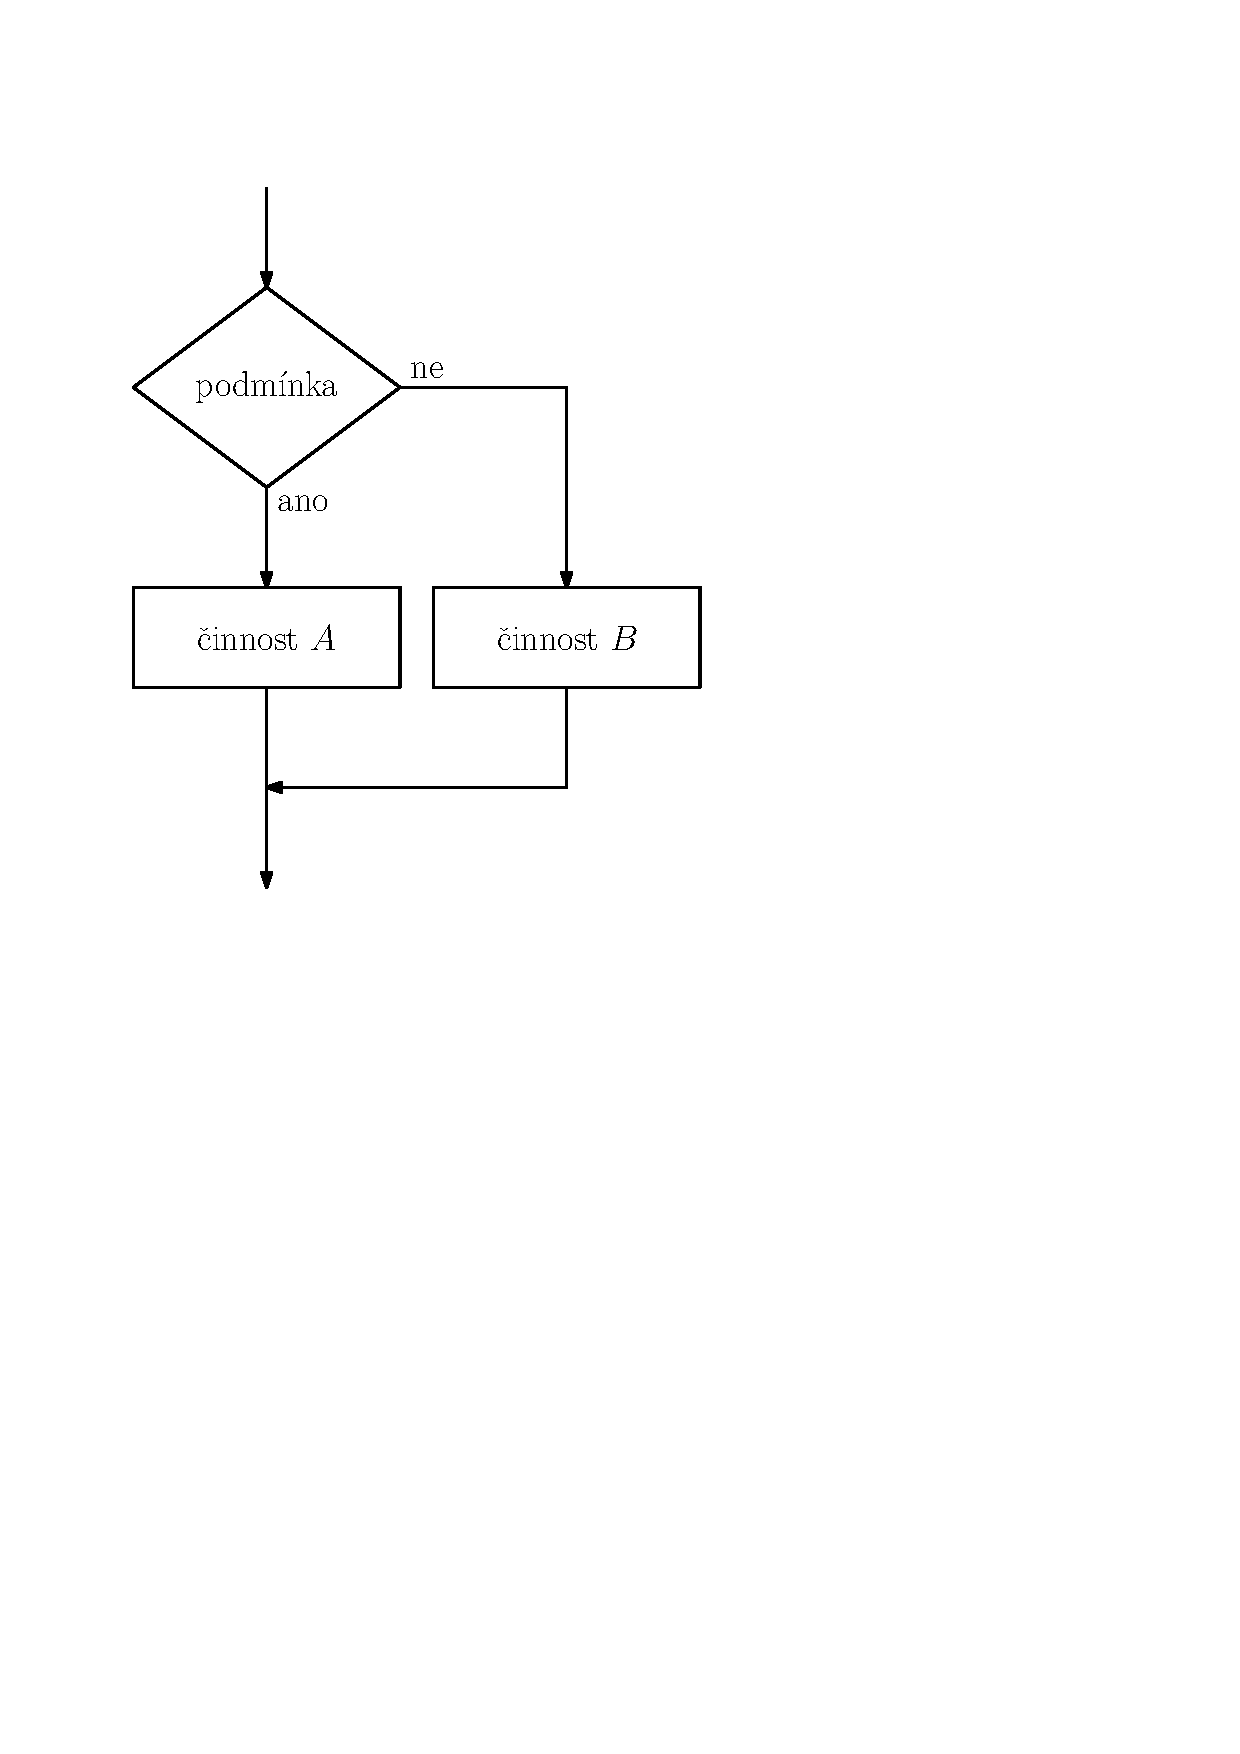
\includegraphics[scale=.5]{../images/00-vyvojak-selekce.pdf}
                \end{figure}
            \end{column}
            \begin{column}{.5\textwidth}
                \begin{figure}
                    \centering
                    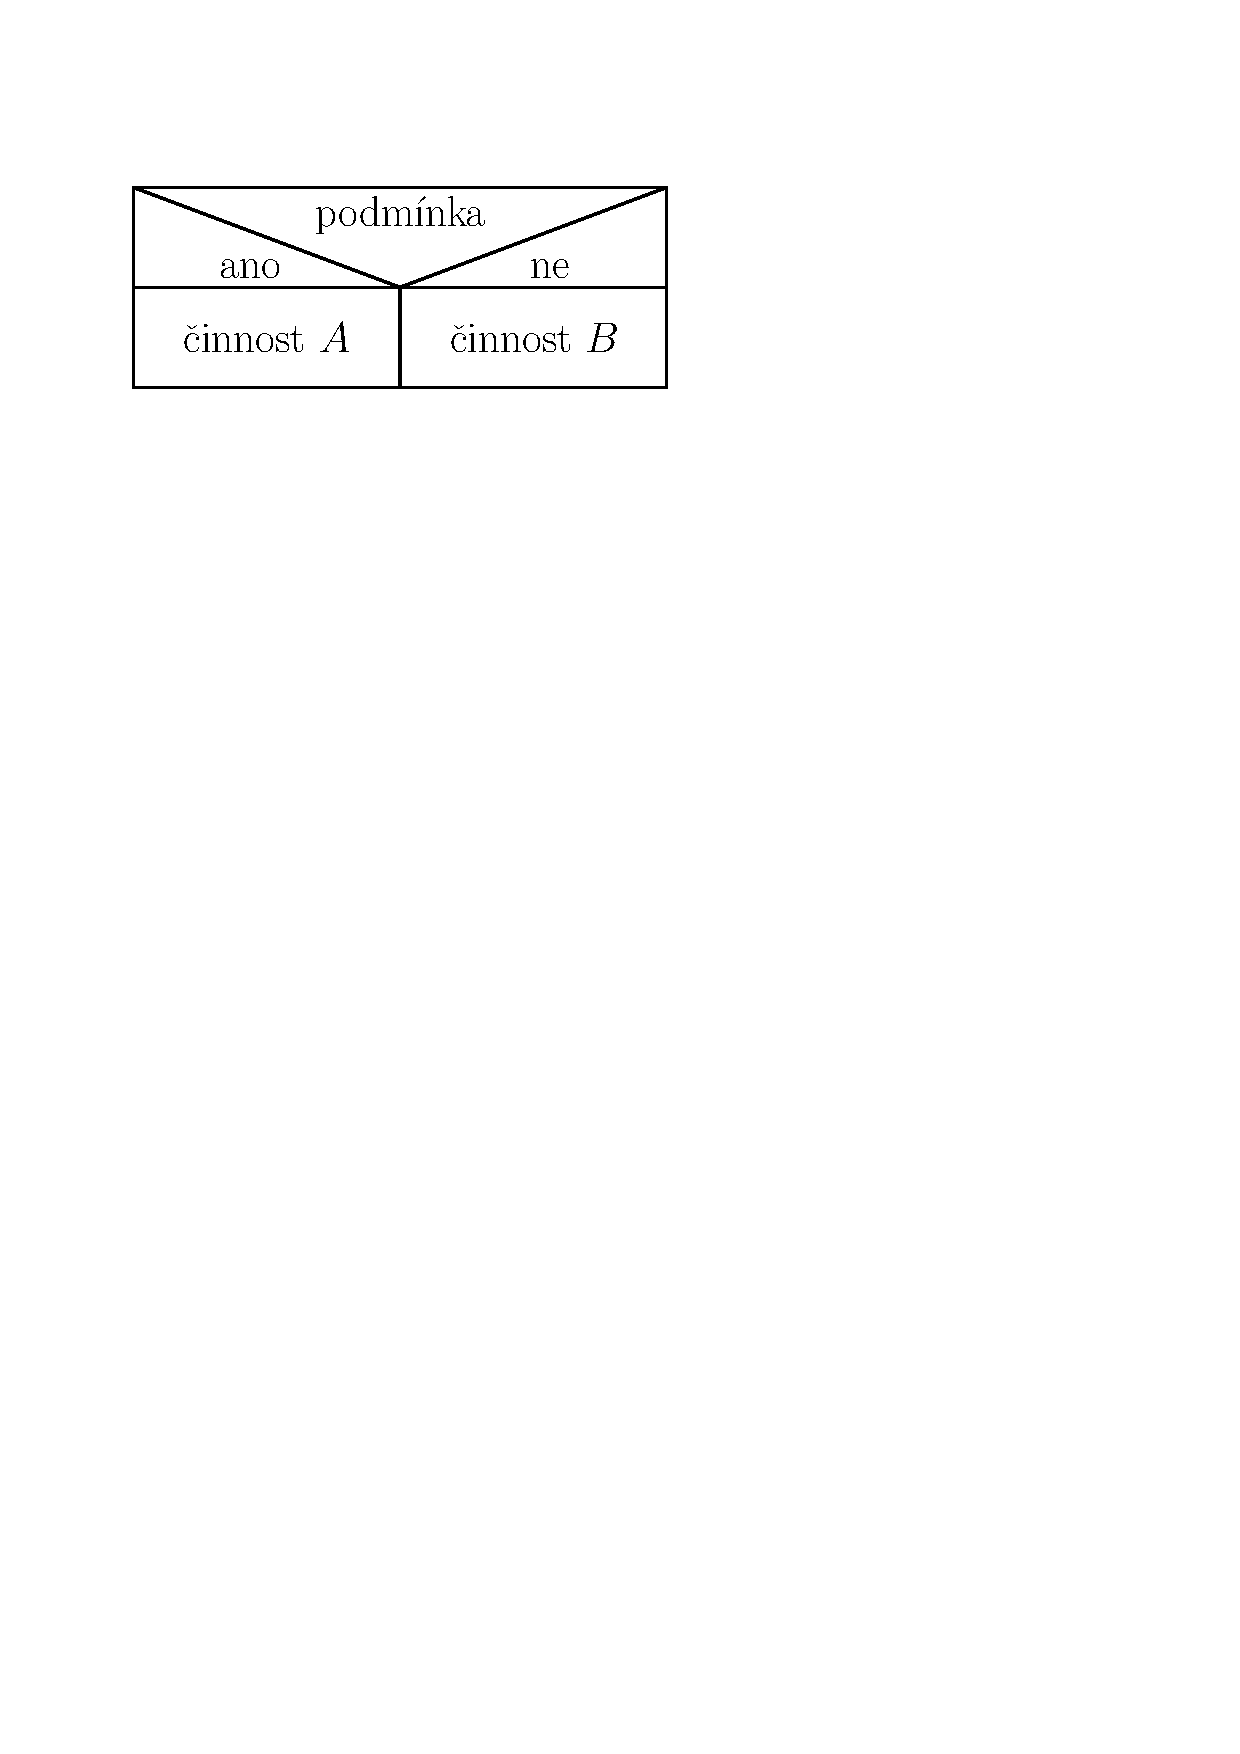
\includegraphics[scale=.5]{../images/00-strukturogram-selekce.pdf}
                \end{figure}
            \end{column}
        \end{columns}
    \end{frame}

    \subsubsection{Iterace s testem na začátku}
    \begin{frame}{Iterace s testem na začátku}
        \begin{columns}
            \begin{column}{.5\textwidth}
                \begin{figure}
                    \centering
                    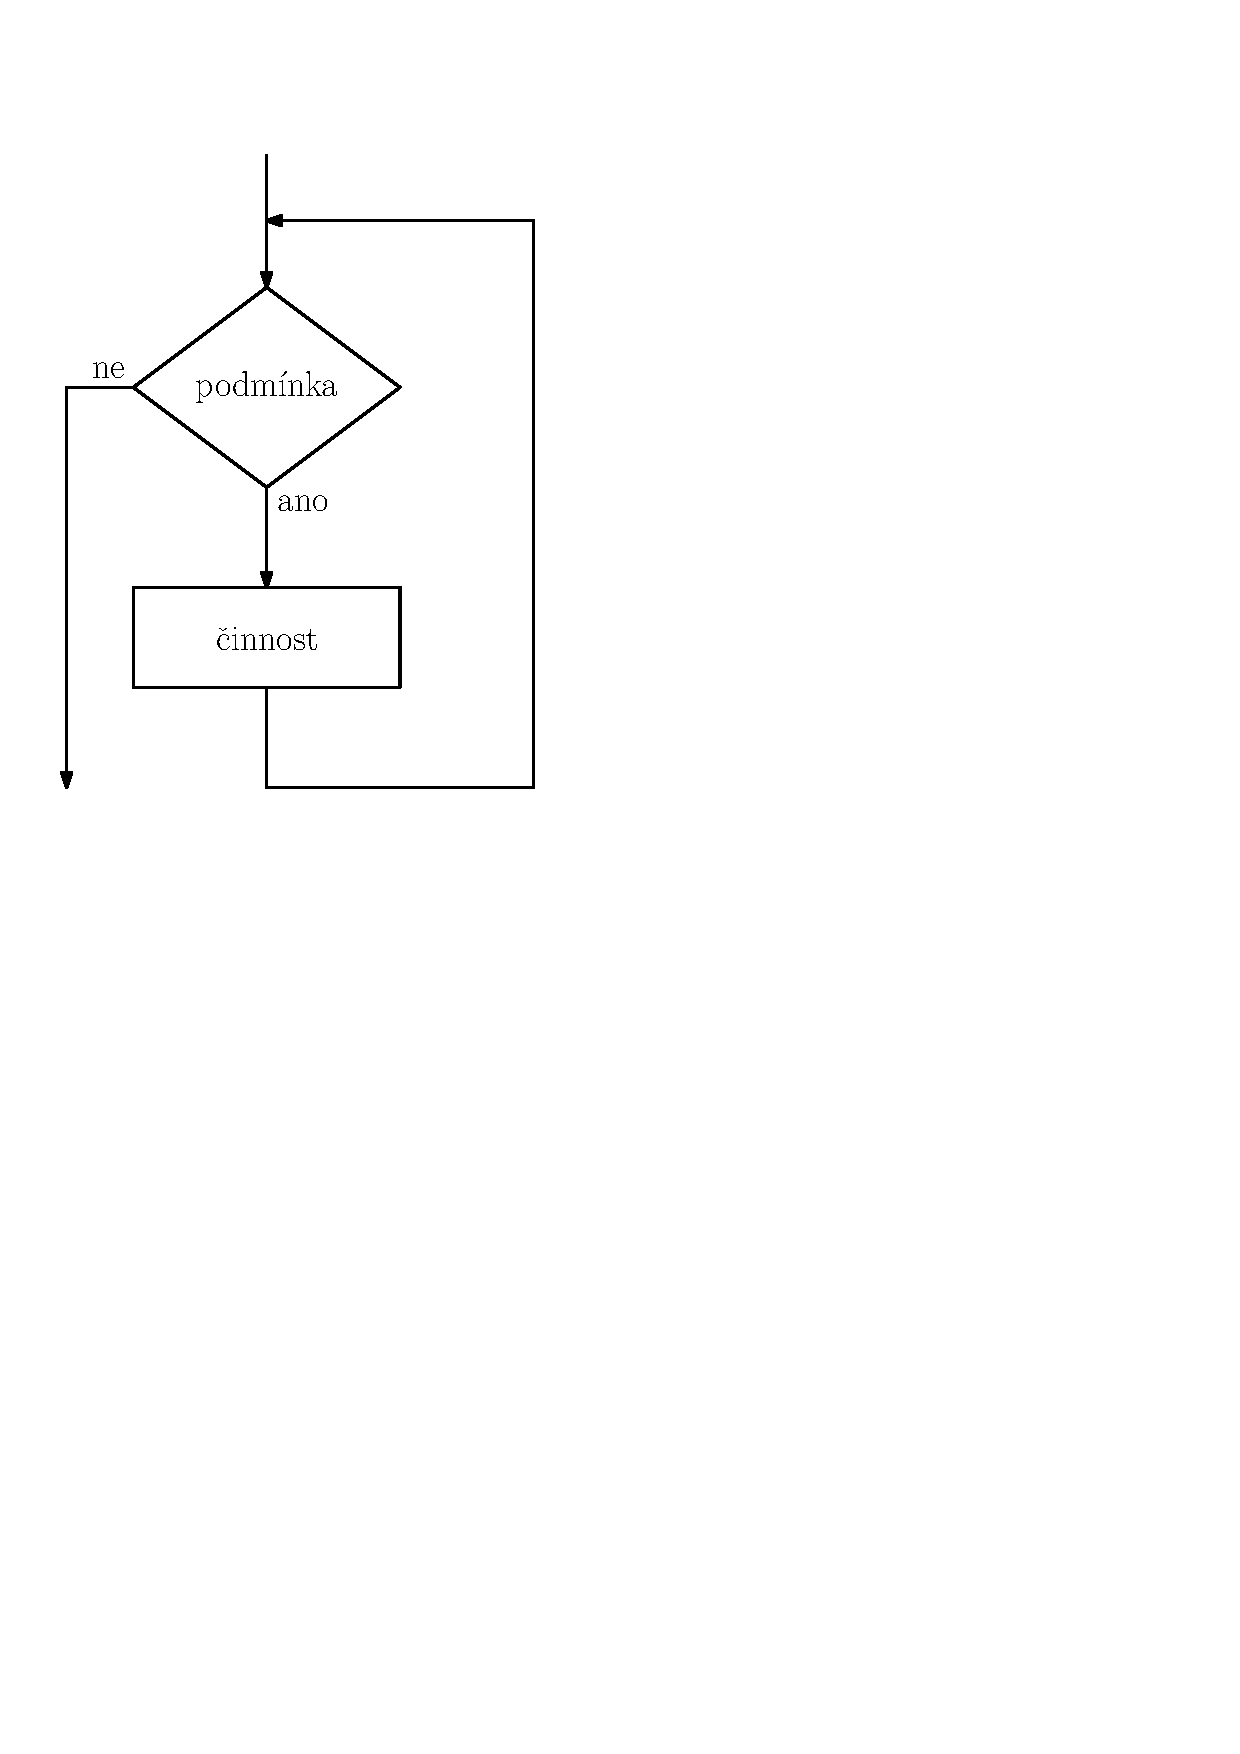
\includegraphics[scale=.5]{../images/00-vyvojak-iterace-zacatek.pdf}
                \end{figure}
            \end{column}
            \begin{column}{.5\textwidth}
                \begin{figure}
                    \centering
                    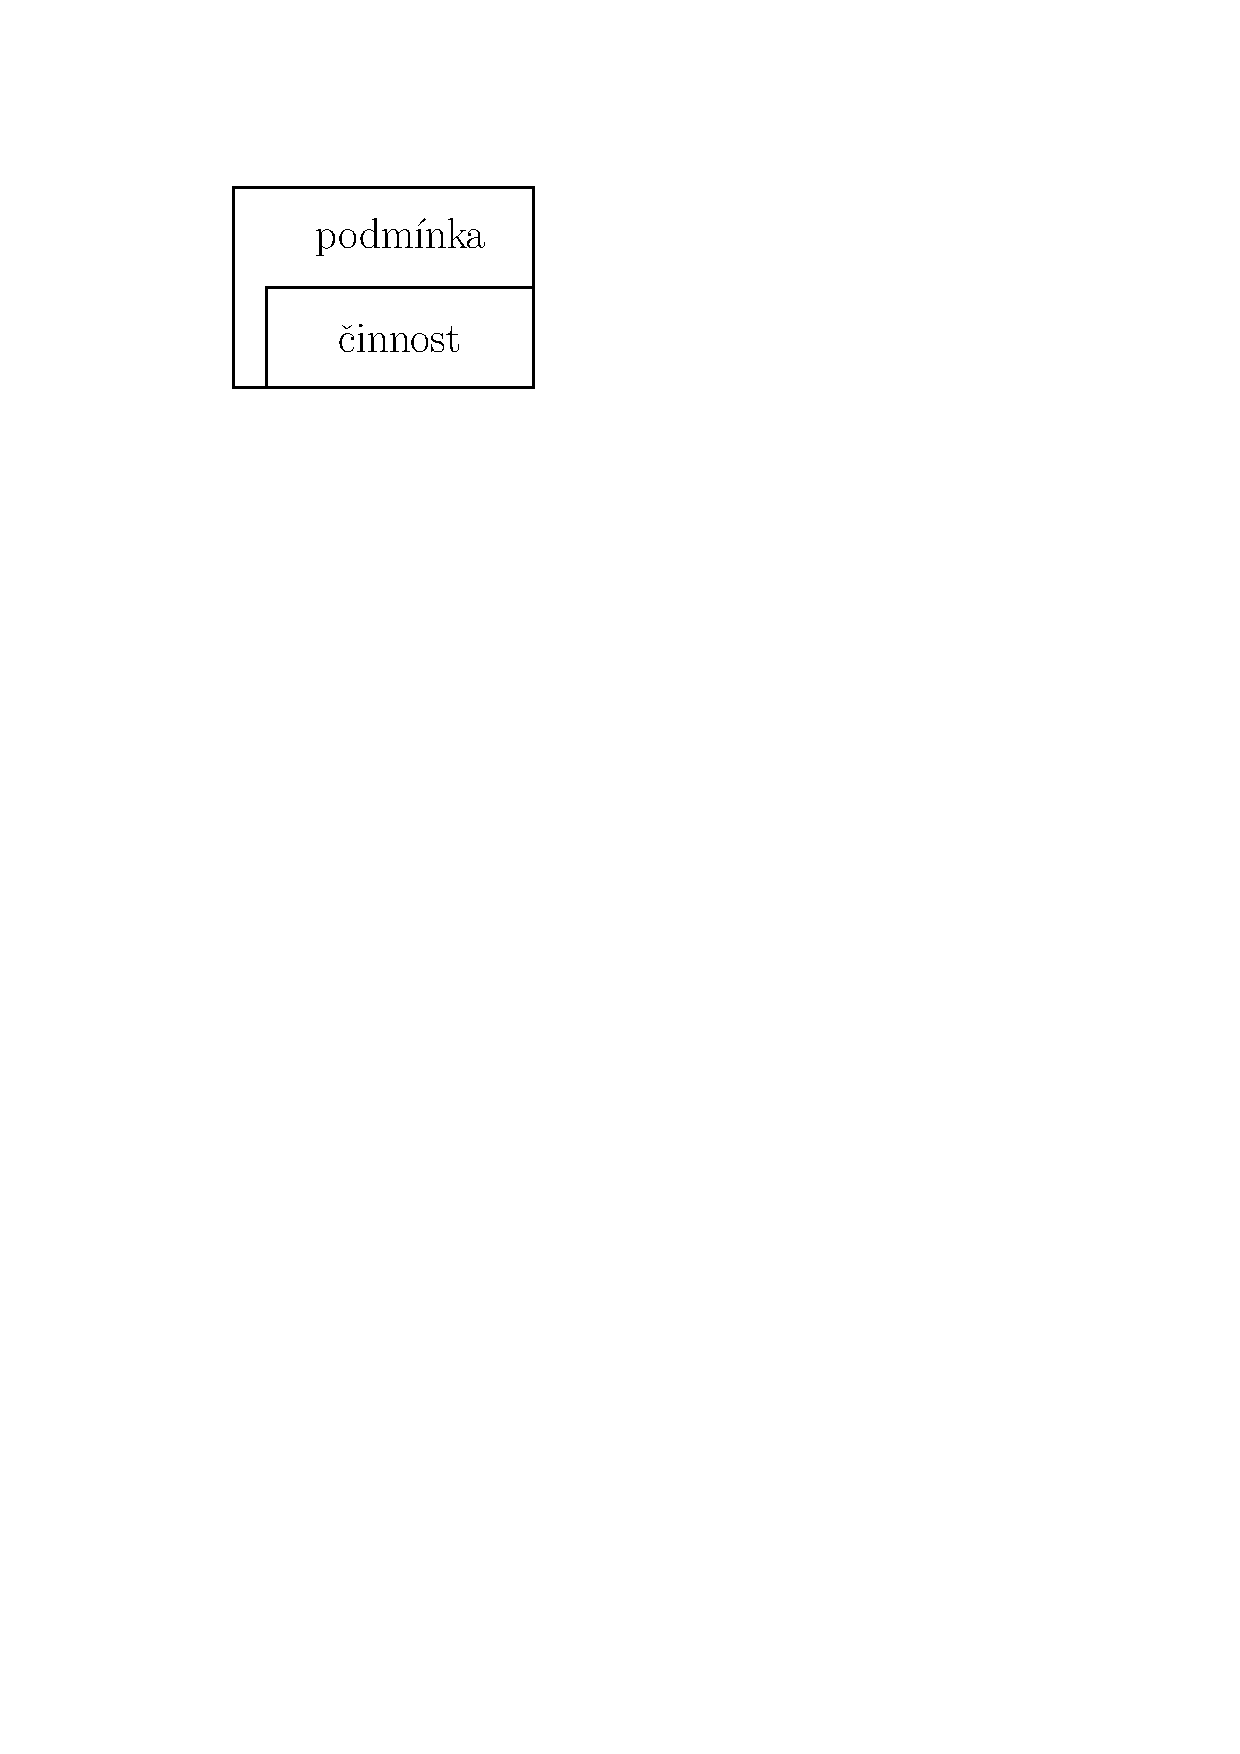
\includegraphics[scale=.5]{../images/00-strukturogram-iterace-zacatek.pdf}
                \end{figure}
            \end{column}
        \end{columns}
    \end{frame}

    \subsubsection{Iterace s testem na konci}
    \begin{frame}{Iterace s testem na konci}
        Oproti iteraci s testem na začátku je zde zaručeno, že tělo iterace se vykoná \textbf{alespoň jednou}.
        \begin{columns}
            \begin{column}{.5\textwidth}
                \begin{figure}
                    \centering
                    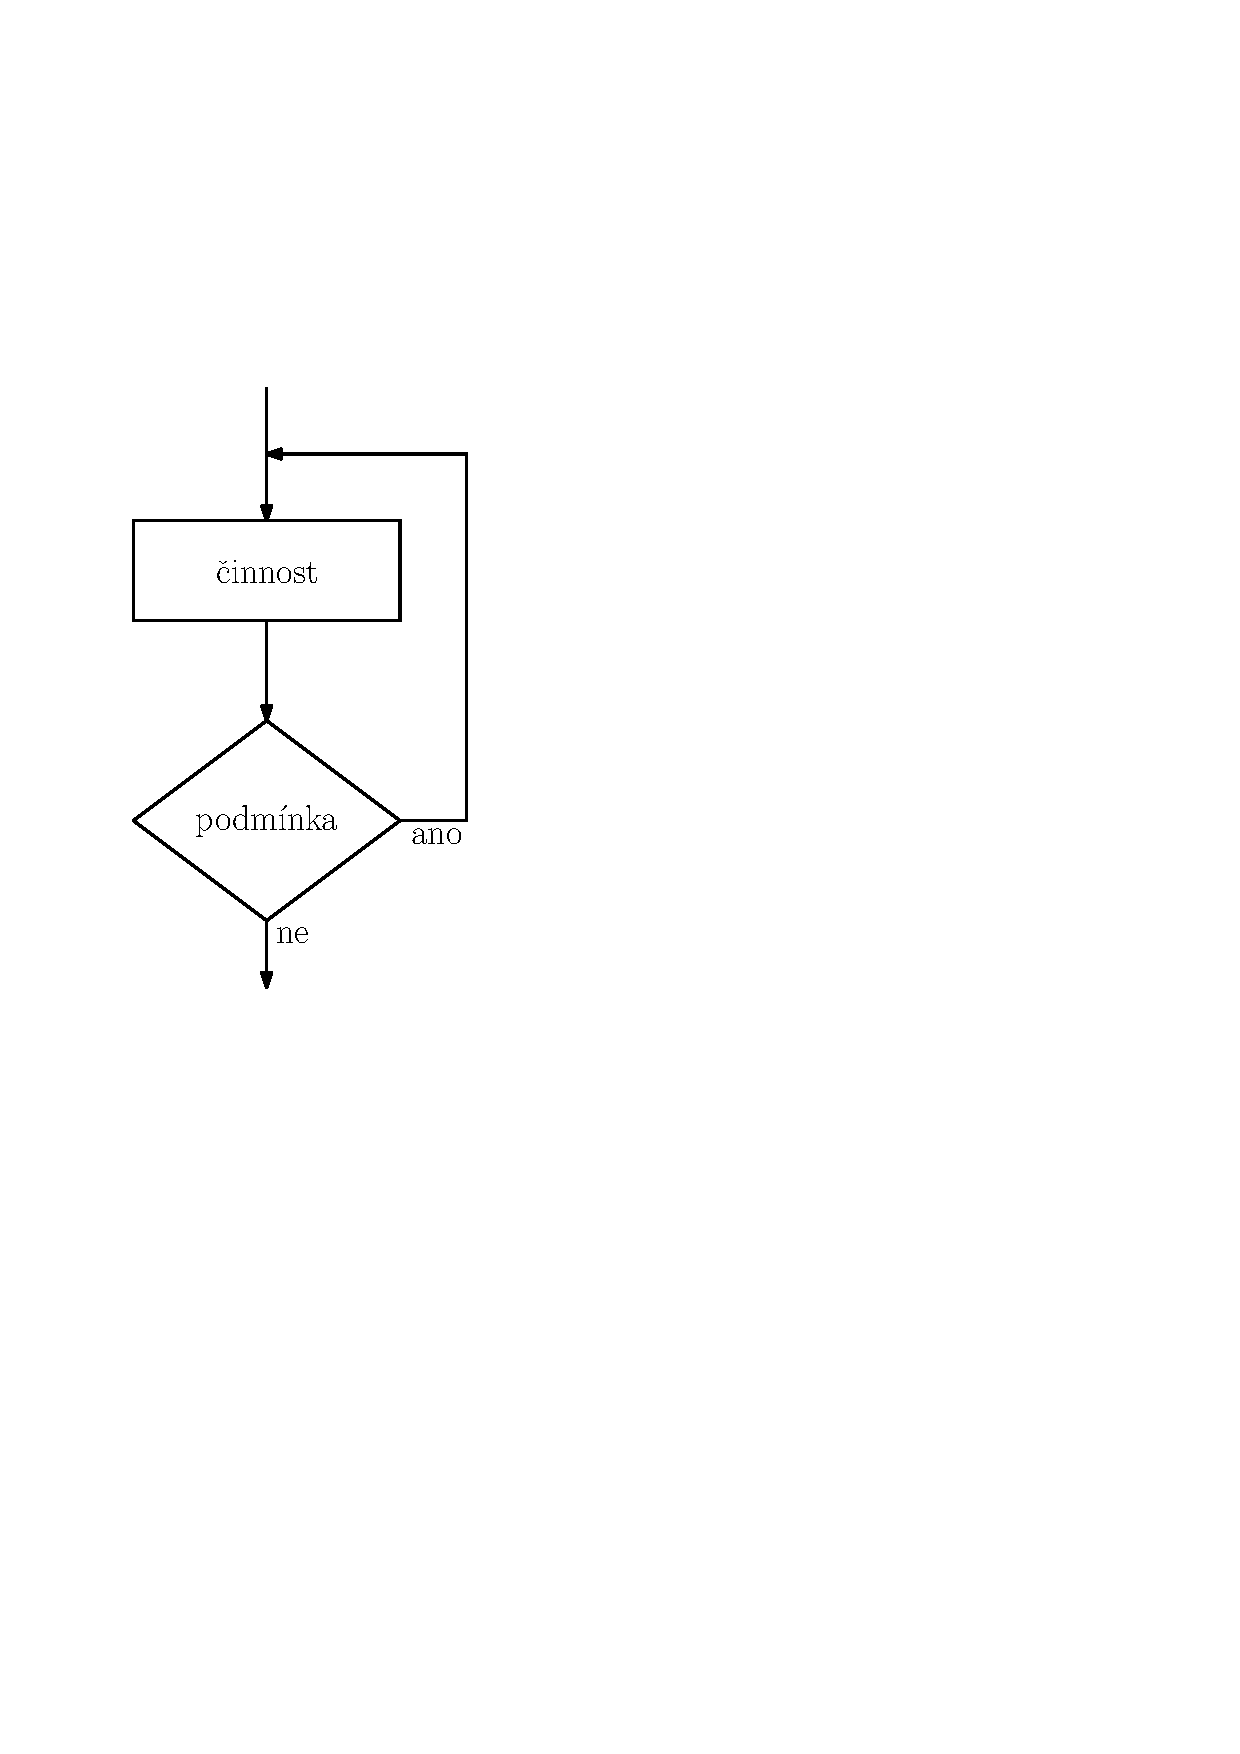
\includegraphics[scale=.5]{../images/00-vyvojak-iterace-konec.pdf}
                \end{figure}
            \end{column}
            \begin{column}{.5\textwidth}
                \begin{figure}
                    \centering
                    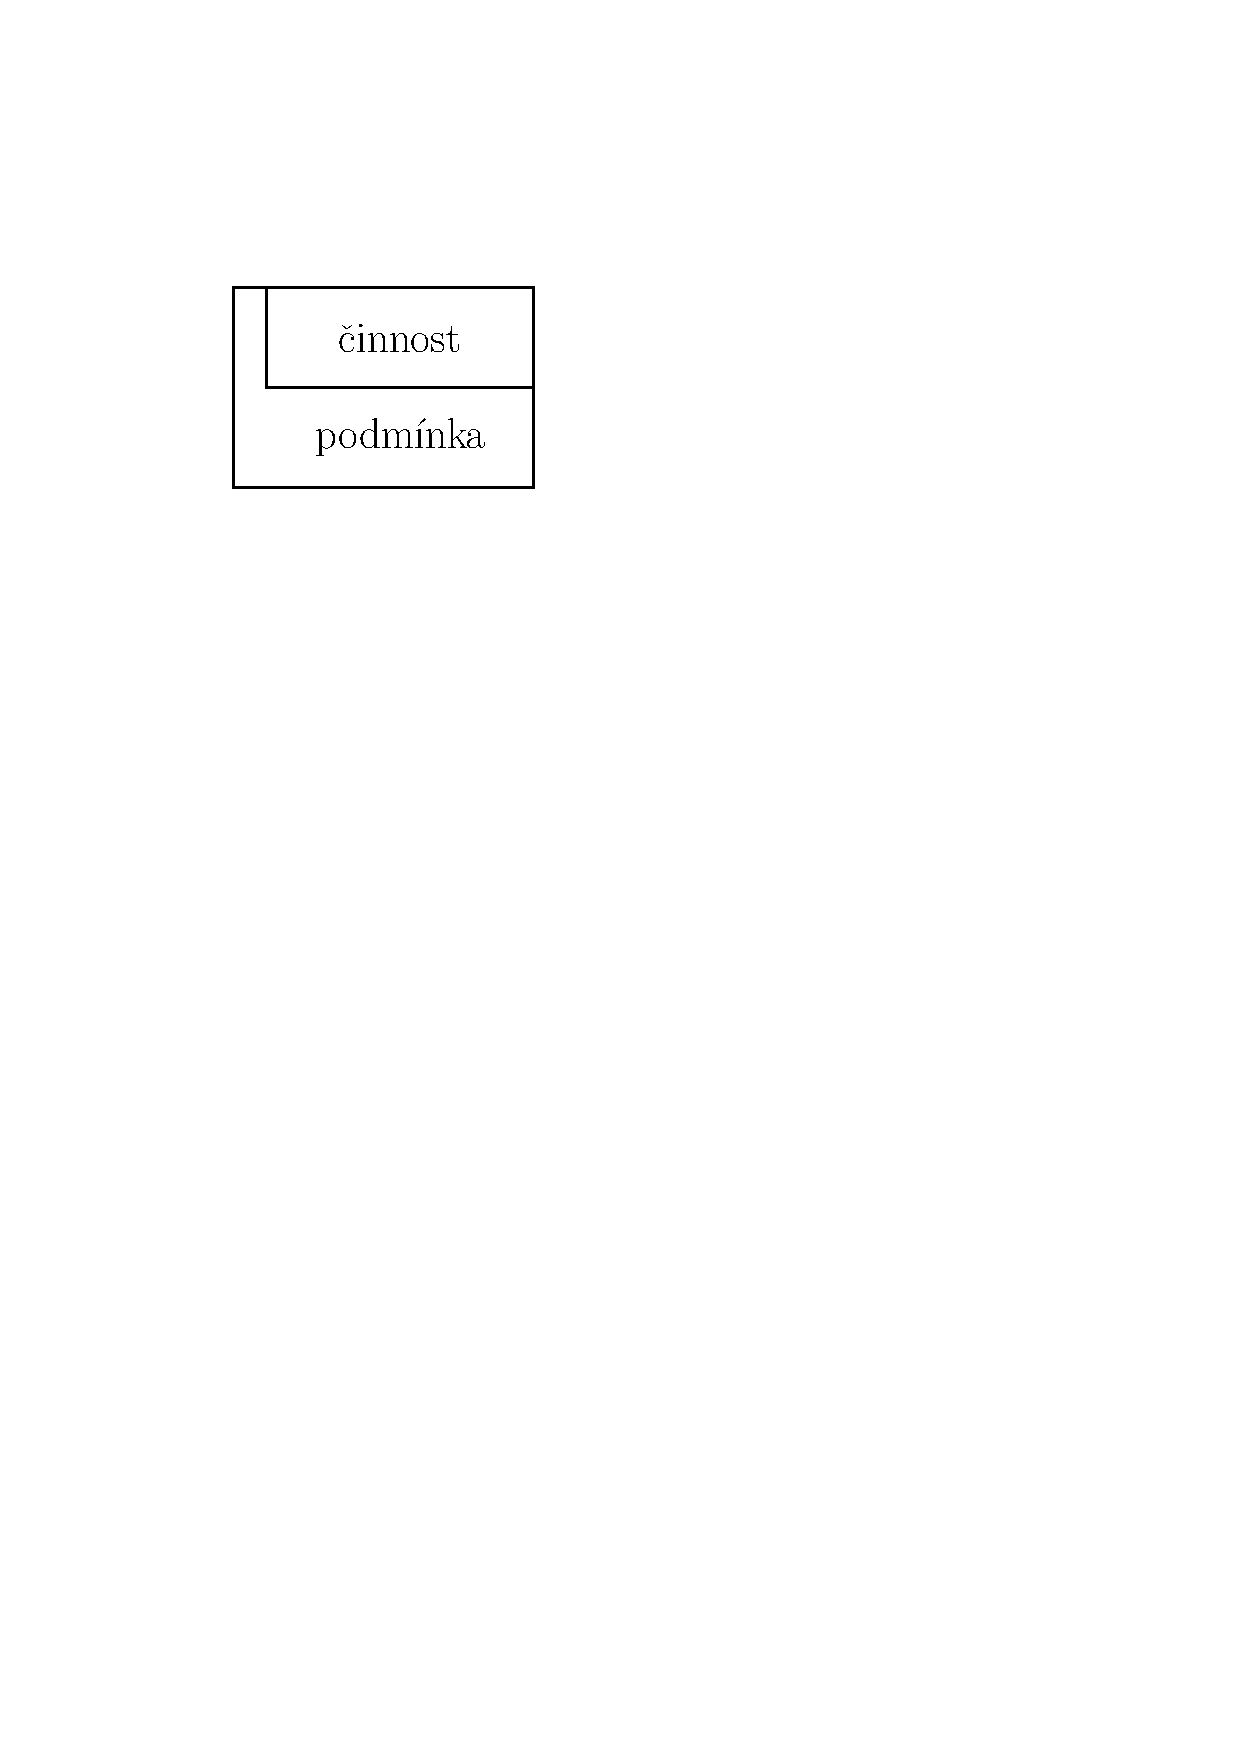
\includegraphics[scale=.5]{../images/00-strukturogram-iterace-konec.pdf}
                \end{figure}
            \end{column}
        \end{columns}
    \end{frame}

    \section{Závěr}
    \begin{frame}{Dotazy?}
        \begin{figure}
            \centering
            
\includegraphics[scale=.5]{../images/discussion.pdf}
        \end{figure}
    \end{frame}

\end{document}